\documentclass{beamer}
\usepackage{lipsum}
\usepackage[brazilian]{babel}
\usepackage[utf8]{inputenc}

\usepackage{enumerate}
\usepackage{dcolumn}
\usepackage{tabu}
\usepackage{colortbl}
\usepackage{booktabs}
\usepackage{changes}
\usepackage{listings}
\usepackage{placeins}
\usepackage{amsmath}

\usepackage{multirow}

\newcommand*{\Scale}[2][4]{\scalebox{#1}{$#2$}}%
\newcommand*{\Resize}[2]{\resizebox{#1}{!}{$#2$}}%

\usetheme[faculty=ppca,language=logo,framenumber,totalframenumber]{UniversiteitGent}

\title{Desenvolvimento de Microserviços \\ no CPD/UnB }
\subtitle{ \textcolor{forestgreen}{Universidade de Brasília} \\
			\textcolor{black}{Centro de Informática} \\
			4 de Dezembro de 2017
}
\author{Everton de Vargas Agilar \\
		evertonagilar@unb.br
}



\begin{document}

\begin{frame}
  \titlepage
\end{frame}




%%##############################################################




\subsection{Plan}

\begin{frame}
  \frametitle{Plano}

    \begin{itemize}

	    \item<1-> Nova Arquitetura de Desenvolvimento do CPD/UnB
		    \begin{itemize}
				\item<1->Motivação para adoção de SOA
				\item<1->Ferramentas e tecnologias adotadas e desenvolvidas
				\item<1->ErlangMS -- Plataforma agnóstica de serviços
			\end{itemize}

  	  	\item<1-> Implementação de Serviços e Microserviços
		    \begin{itemize}
				\item<1->Desenvolvimento de serviços em Java
				\item<1->Autenticação de usuários com o proxy LDAP
				\item<1->Autenticação e autorização de serviços REST com OAuth2
  		     \end{itemize}
 	  
	   	\item<1-> Pontos Positivos e Desafios
	   	  
    \end{itemize}

\end{frame}



\begin{frame}
\frametitle{Motivação para adoção de SOA}

\begin{itemize}
	\item<1->Maximizar o reuso dos fluxos de negócios;
	\item<1->Modernizar os sistemas de maneira sistemática e incremental;
	\item<1->Minimizar dependências tecnológicas; 
	\item<1->Experimentar SOA (Service Oriented Architecture).
\end{itemize}

\end{frame}


\begin{frame}
\frametitle{Ferramentas e tecnologias adotadas}

\begin{figure}
	\centering
	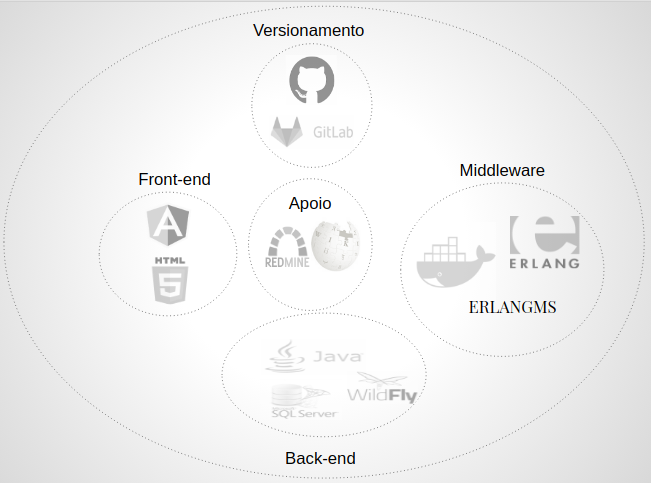
\includegraphics[scale=0.25]{img/tec.png}
\end{figure}

\end{frame}


%%##############################################################




\section{Introdução}


\subsection{Introdução}


%%##############################################################




\subsection{Sobre}


\begin{frame}
  \frametitle{ErlangMS -- Plataforma agnóstica de serviços}

  \begin{exampleblock}{ERLANGMS}
  
É uma plataforma de software desenvolvida para facilitar a integração de sistemas por meio de um barramento 
de serviços orientado a contratos de serviços + SDK + Processo de modernização e arquitetura documentado (SMSOC).

  \end{exampleblock}

  
\end{frame}


\begin{frame}
  \frametitle{ErlangMS -- Plataforma agnóstica de serviços}

  \begin{exampleblock}{Características do barramento}
  
	  \begin{itemize}
		\item<1->Multiplataforma e modular;
	    \item<1->Serviços especificados em catálogos de serviços;
	    \item<1->Suporta serviços RESTful com alta escalabilidade;
   	    \item<1->Modelo de concorrência: Actor Model;
   	    \item<1->Integração com back-end via SDK e Data loaders;
		\item<1->Implementação de web services em Erlang e Java;
	  \end{itemize}

  \end{exampleblock}

  
\end{frame}


\begin{frame}
  \frametitle{ErlangMS -- Plataforma agnóstica de serviços}

  \begin{exampleblock}{Características do barramento}
  
	  \begin{itemize}
		\item<1->HTTP/2, HTTP/1.1, HTTPS (Secure TLS Listener);
	    \item<1->LDAP v3 -- Proxy LDAP;
	    \item<1->HTTP Basic authentication;
    	    \item<1->OAuth2 authentication;
		\item<1->Api query -- filter, fields, sort, limit.
	  \end{itemize}

  \end{exampleblock}

  
\end{frame}


  
\end{frame}



\section{Principais Resultados do Trabalho}


\begin{frame}[c]{ }
\centering
  \huge{Principais Resultados do Trabalho}
\end{frame}



\begin{frame}
  \frametitle{Desenvolvimento de serviços em Java}

	\begin{figure}
	\centering
		
\includegraphics[scale=0.2]{img/sdk.png}
	\end{figure}

	  \begin{itemize}
		\item<1->Saldo do RU. Uso: https://matriculaweb.unb.br
	    \item<1->Consulta foto de aluno. Uso: sistemas que exibem fotos
	    \item<1->Declaração de aluno regular
   	    \item<1->Declaração nada consta. Uso: http://www.sgp.unb.br
   	    \item<1->Conj. web services para o CIC
		\item<1->Conj. web services para novos sistemas (Questionario, SAE)
	  \end{itemize}
  
\end{frame}


\begin{frame}
  \frametitle{Autenticação de usuários com proxy LDAP}

	\begin{figure}
	\centering
		
\includegraphics[scale=0.3]{img/ldap.png}
	\end{figure}


	  \begin{itemize}
		\item<1->Sistema Eletrônico de Informações (SEI)
	    \item<1->Sistema de Inscrição Pós-Graduação
	    \item<1->Redmine
	  \end{itemize}
  
\end{frame}


\begin{frame}
  \frametitle{Autenticação/autorização OAuth2}

	\begin{figure}
	\centering
		
\includegraphics[scale=0.2]{img/oauth2.png}
	\end{figure}

	  \begin{itemize}
		\item<1->Integração com sistema de controle de acesso (SCA)
	    \item<1->Permite autenticar e autorizar chamadas REST
	    \item<1->Single sign on
	  \end{itemize}
  
\end{frame}



\begin{frame}
  \frametitle{Pontos Positivos e Desafios}

  \begin{exampleblock}{Pontos Positivos}
  
	  \begin{itemize}
 	    \item<1->O CPD consegue atender demandas que na arquitetura anterior 
				 era muito difícil ou praticamente impossível devido as questões de segurança e acesso a banco de dados;
		\item<1->Sistemas menores e mais leves;
		\item<1->Cultura Devops.
	  \end{itemize}

  \end{exampleblock}


  \begin{exampleblock}{Desafios}
  
	  \begin{itemize}
 	    \item<1->Complexidade operacional;
		\item<1->Gerenciamento dos catálogos de serviços;
		\item<1->Monitoramento dos serviços em uso.
	  \end{itemize}

  \end{exampleblock}

  
\end{frame}


\begin{frame}[c]{ }
\centering
  \huge{Obrigado!}
\end{frame}


\end{document}



